\documentclass[a4paper,14pt]{extarticle}

\usepackage[utf8x]{inputenc}
\usepackage[T1]{fontenc}
\usepackage[russian]{babel}
\usepackage{hyperref}
\usepackage{indentfirst}
\usepackage{here}
\usepackage{array}
\usepackage{graphicx}
\usepackage{caption}
\usepackage{subcaption}
\usepackage{chngcntr}
\usepackage{amsmath}
\usepackage{amssymb}
\usepackage[left=2cm,right=2cm,top=2cm,bottom=2cm,bindingoffset=0cm]{geometry}
\usepackage{multicol}
\usepackage{multirow}
\usepackage{titlesec}
\usepackage{listings}
\usepackage{color}
\usepackage{enumitem}
\usepackage{cmap}
\usepackage{url}

\definecolor{green}{rgb}{0,0.6,0}
\definecolor{gray}{rgb}{0.5,0.5,0.5}
\definecolor{purple}{rgb}{0.58,0,0.82}

\lstdefinelanguage{none}{}

\lstset{
	language={none},
	inputpath={../logs/},
	backgroundcolor=\color{white},
	commentstyle=\color{green},
	keywordstyle=\color{blue},
	numberstyle=\color{gray}\scriptsize\ttfamily,
	stringstyle=\color{purple},
	basicstyle=\footnotesize\ttfamily,
	breakatwhitespace=false,
	breaklines=true,
	captionpos=b,
	keepspaces=true,
	numbers=left,
	numbersep=5pt,
	showspaces=false,
	showstringspaces=false,
	showtabs=false,
	tabsize=4,
	frame=single,
	morekeywords={},
	deletekeywords={},
	extendedchars=false,
	columns=fullflexible,
	literate=%
		{~}{{\raise.25ex\hbox{$\mathtt{\sim}$}}}{1}%
		{-}{-}{1}
}

\titleformat*{\section}{\large\bfseries} 
\titleformat*{\subsection}{\normalsize\bfseries} 
\titleformat*{\subsubsection}{\normalsize\bfseries} 
\titleformat*{\paragraph}{\normalsize\bfseries} 
\titleformat*{\subparagraph}{\normalsize\bfseries} 

\counterwithin{figure}{section}
\counterwithin{equation}{section}
\counterwithin{table}{section}
\newcommand{\sign}[1][5cm]{\makebox[#1]{\hrulefill}}
\newcommand{\equipollence}{\quad\Leftrightarrow\quad}
\newcommand{\no}[1]{\overline{#1}}
\graphicspath{{../pics/}}
\captionsetup{justification=centering,margin=1cm}
\def\arraystretch{1.3}
\setlength\parindent{5ex}
\titlelabel{\thetitle.\quad}

\setitemize{topsep=0em, itemsep=0em}
\setenumerate{topsep=0em, itemsep=0em}

\begin{document}

\begin{titlepage}
\begin{center}
	Санкт-Петербургский Политехнический Университет Петра Великого\\[0.3cm]
	Институт компьютерных наук и технологий \\[0.3cm]
	Кафедра компьютерных систем и программных технологий\\[4cm]
	
	\textbf{ОТЧЕТ}\\ 
	\textbf{по лабораторной работе}\\[0.5cm]
	\textbf{<<Data Mining>>}\\[0.1cm]
	Интеллектуальные системы\\[3.0cm]
\end{center}

\begin{flushright}
	\begin{minipage}{0.5\textwidth}
		\textbf{Работу выполнил студент}\\[3mm]
		гр. 3540901/91502 \hfill \sign[1.1cm] \hfill Дьячков В.В.\\[5mm]
		\textbf{Работу принял преподаватель}\\[5mm]
		\sign[2.1cm] \hfill к.т.н., доц. Бендерская Е.Н. \\[5mm]
	\end{minipage}
\end{flushright}

\vfill

\begin{center}
	Санкт-Петербург\\[0.3cm]
	\the\year
\end{center}
\end{titlepage}

\addtocounter{page}{1}

\tableofcontents
\newpage

\section{Программа работы}

\begin{enumerate}
	\item На примере одной из экспертных систем ExSys Corvid\cite{corvid-demos} укажите содержание компонентов:
	\begin{itemize}
		\item Диалоговый компонент
		\item База данных
		\item База знаний
		\item Решатель
	\end{itemize}
	\item Выполните лабораторные работы 1-6 из методических рекомендаций Д.И. Муромцев. Оболочка экспертных систем Exsys Corvid – СПб: СПб ГУ ИТМО, 2006 \cite{labs}.
	\item По приведенному описанию ЭС разработайте статическую экспертную систему для нахождения характерных неисправностей прибора Диск-250 ДД и метода их решения. Прибор показывающий и регистрирующий Диск-250 ДД предназначен для измерения и регистрации силы тока, а также неэлектрических величин, преобразованных в силу тока. Данная ЭС предназначена для использования слесарями в целях быстрого обнаружения неисправности и ее устранения. Привести в отчете:
	\begin{itemize}
		\item Перечень переменных с описанием их типа и значений;
		\item Дерево решений, разработанной Вами ЭС;
		\item Базу знаний, разработанной Вами ЭС;
		\item Интерфейс с пользователем (перечень вопросов, задаваемых пользователю).
	\end{itemize}
\end{enumerate}

\newpage

\section{Выполнение работы}

\subsection{Компоненты экспертной системы}

Рассмотрим компоненты ЭС на примере системы для выбора породы собаки по ряду вопросов, связанных с уходом за собакой, привычками человека и т.д.\footnote{\url{http://www.exsyssoftware.com/CORVID/corvidsr?KBNAME=../Dogs/Dogs.CVR}}
\begin{itemize}
	\item Диалоговый компонент: Java Applet
	\item База данных: Список пород собак и особенности их содержания и поведения собак
	\item База знаний: Набор статических инструкций о различных породах
	\item Решатель: Формирователь правил, которые приводят к подбору подходящего ресторана. Данные для решения берутся из БД и БЗ.
\end{itemize}

\section{Лабораторные работы по CORVID}

\subsection{Создание простейшей системы}

В рамках данной работы создадим простейшую ЭС для принятия решения о замене лампочки в том случае, если она перегорела. На рис. \ref{fig:bulb_1} приведен логический блок разработанной ЭС.

\begin{figure}[H]
	\centering
	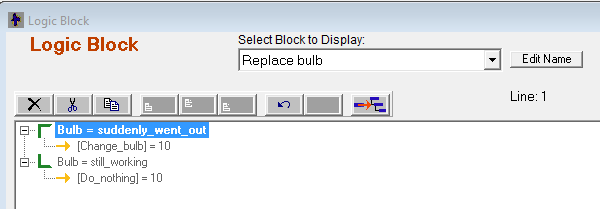
\includegraphics[width=0.9\linewidth]{bulb_1}
	\caption{Логический блок ЭС}
	\label{fig:bulb_1}
\end{figure}

В листинге \ref{lst:bulb_1} приведен сгенерированный алгоритм работы ЭС.

\begin{lstlisting}[label=lst:bulb_1, caption={Алгоритм работы ЭС}]
IF:
	Bulb in your house suddenly went out
THEN:
	Change the bulb: Confidence = 10

IF:
	Bulb in your house still working
THEN:
	Do nothing: Confidence = 10
\end{lstlisting}

На рис. \ref{fig:bulb_2} приведен пользовательский интерфейс ЭС.

\begin{figure}[H]
	\centering
	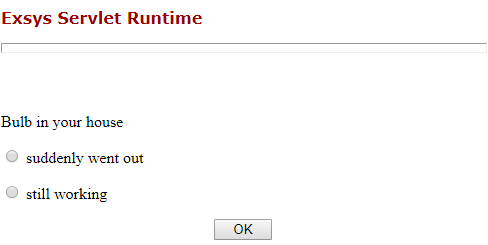
\includegraphics[width=0.7\linewidth]{bulb_2}
	\caption{Пользовательский интерфейс ЭС}
	\label{fig:bulb_2}
\end{figure}

На рис. \ref{fig:bulb_3} приведены результаты работы ЭС.

\begin{figure}[H]
	\centering
	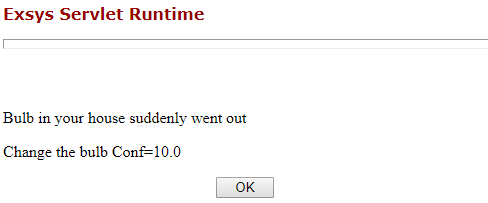
\includegraphics[width=0.7\linewidth]{bulb_3}
	\caption{Результаты работы ЭС}
	\label{fig:bulb_3}
\end{figure}

Таким образом, в рамках работы изучен интерфейс Exsys CORVID на примере простейшей экспертной системы.

\subsection{Улучшение интерфейса пользователя}

В рамках данной работы рассмотрим возможности форматирования интерфейса в системе Exsys CORVID.

На рис. \ref{fig:bulb_4} приведено изображение обновленного окна результатов. Был изменен шрифт и оставлено отображение только текстового значения.

\begin{figure}[H]
	\centering
	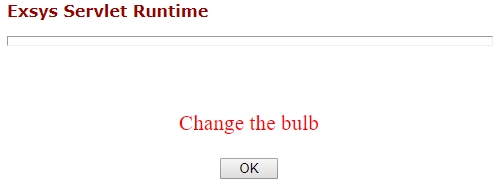
\includegraphics[width=0.7\linewidth]{bulb_4}
	\caption{Результаты работы ЭС}
	\label{fig:bulb_4}
\end{figure}

Заменить отображение вопроса на изображение не удалось по известным только разработчикам Exsys CORVID причинам.

\subsection{Усиление логики системы}

В рамках данной работы усовершенствуем логический блок имеющийся ЭС. Были добавлены дополнительные переменные:
\begin{itemize}
	\item \code{OTHER_LIGHTS_IN_THE_HOUSE} -- переменная используется при запросе
	у пользователя, погасли ли другие лампочки в комнате.
	\item \code{OTHER_LIGHTS_IN_THE_ROOM} -- используется при запросе у
	пользователя, погасли ли другие лампочки в доме.
	\item \code{FIX_CIRCUIT_BREAKER} -- рекомендация для случая, когда проблема
	заключается в сломанном выключателе (предохранителе).
	\item \code{CALL_THE_POWER_COMPANY} -- рекомендация в случае отключения
	электричества.
\end{itemize}

При помощи приемом, разобранных выше, был изменен логический блок ЭС. Итоговые правила ЭС приведены ниже.

\begin{lstlisting}[caption={Алгоритм работы ЭС}]
IF:
	Bulb in your house suddenly went out
AND:
	The other lights in the room stay on
THEN:
	Change the bulb: Confidence = 10

IF:
	Bulb in your house suddenly went out
AND:
	The other lights in the room go out
AND:
	The other lights in the house stay on
THEN:
	Check the circuit breaker for the room and reset any tripped breakers: Confidence = 10

IF:
	Bulb in your house suddenly went out
AND:
	The other lights in the room go out
AND:
	The other lights in the house go out
THEN:
	Call the power company and report the problem: Confidence = 10

IF:
	Bulb in your house still working
THEN:
	Do nothing: Confidence = 10
\end{lstlisting}

ЭС была протестирована при разных ответах. 

\begin{figure}[H]
	\centering
	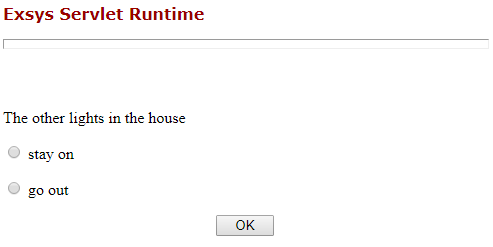
\includegraphics[width=0.7\linewidth]{bulb_5}
	\caption{Дополнительный вопрос ЭС}
\end{figure}

\begin{figure}[H]
	\centering
	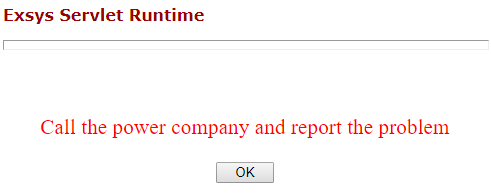
\includegraphics[width=0.7\linewidth]{bulb_6}
	\caption{Результат работы ЭС}
\end{figure}

Таким образом, в имеющейся экспертной системе успешно выполнено усиление логики в результате обработки различных случаев отключения лампочек (одной, во всей комнате, во всем доме).

\subsection{Обратная связь}

В рамках данной работы был рассмотрен механизм обратной связи. В случае, когда системе необходимо узнать значение переменной, и существует правило которое разрешает ей устанавливать значения для этой переменной, система автоматически достроит до конца правило, установив значение этой переменной. 

Для этого был добавлен дополнительный логический блок \code{Radio}. Вместо вопроса "работает ли электричество в доме" система задает наводящий вопрос -- "слышно ли радио". Если ответ положительный, то ЭС делает заключение, что электричество в доме есть. В обратном случае выводов не делается.

Ниже представлен логический блок, который был сделан с использованием дополнительных переменных.

\begin{lstlisting}[caption={Алгоритм работы ЭС}]
IF:
	The radio in the other room Can be heard
THEN:
	The other lights in the house stay on
\end{lstlisting}

Система была протестирована при разных пользовательских ответах. Ниже представлен пример, когда ЭС задает наводящий вопрос.

\begin{figure}[H]
	\centering
	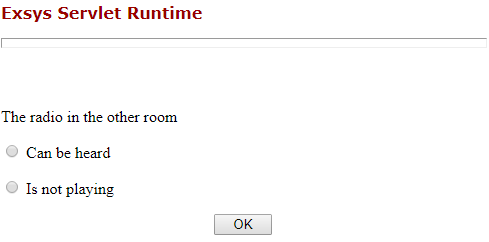
\includegraphics[width=0.7\linewidth]{bulb_7}
	\caption{Наводящий вопрос ЭС}
\end{figure}

\begin{figure}[H]
	\centering
	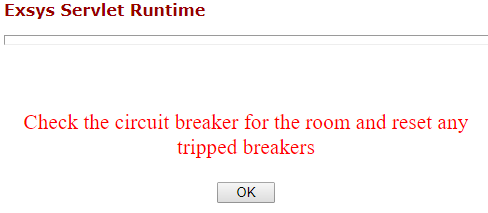
\includegraphics[width=0.7\linewidth]{bulb_8}
	\caption{Результат работы ЭС при положительном ответе на наводящий вопрос}
\end{figure}

Таким образом, в систему добавлена обратная связь, продемонстрирована успешная работа ЭС.

\subsection{Числовые переменные и [[]] подстановки}

Переменные являются основной единицей построения экспертных систем ExSys CORVID. В данной работе был рассмотрен новый тип переменных -- \code{Numeric}. Он был использован для описания мощности лампочки. В систему было добавлено следующее условие: <<если перегоревшая лампочка обладала мощностью менее 75 ватт, то её следует заменить на лампочку такой же мощности; если мощность сгоревшей лампочки более 75 ватт, то она заменяется на лампочку с номиналом 75 ватт.>> Для этого был реализован еще один логический блок \code{Wattage}.

\begin{lstlisting}[caption={Алгоритм работы ЭС}]
IF:
	[Change_bulb] = 10
AND:
	[Wattage] > 75
THEN:
	[Replacement_wattage] = 75

IF:
	[Change_bulb] = 10
AND:
	[Wattage] <= 75
THEN:
	[Replacement_wattage] = [Wattage]
\end{lstlisting}

Система была протестирована на разных пользовательских ответах. Ниже приведен пример, когда мощность лампочки меньше 75 ватт, в следствие чего предложено заменить лампочку на другую с такой же мощностью. Для реализации динамического формирования строки был реализован механизм подстановки переменных \code{[[]]}.

\begin{figure}[H]
	\centering
	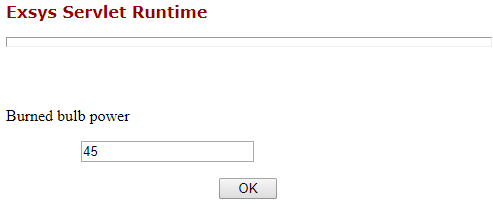
\includegraphics[width=0.7\linewidth]{bulb_9}
	\caption{Запрос числовой переменной}
\end{figure}

\begin{figure}[H]
	\centering
	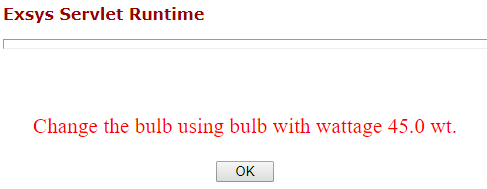
\includegraphics[width=0.7\linewidth]{bulb_10}
	\caption{Информация о мощности нужной лампочки}
\end{figure}

Таким образом, существующая система успешно улучшена рекомендацией о мощности сменной лампочки. Использованы двойные квадратные скобки для включения значения переменной в текст.

\subsection{Переменные коллекции}

В данной работе рассмотрено использование списка переменной длины (\code{Collection}). В этом списке может храниться набор строк, что представит составляемый список покупок. Добавление лампочки в список происходит в случае, когда лампочка должна быть заменена. Для этого был модифицирован логический блок \code{Wattage} как представлено ниже.

\begin{lstlisting}[caption={Алгоритм работы ЭС}]
IF:
	[Change_bulb] = 10
AND:
	[Wattage] > 75
THEN:
	[Replacement_wattage] = 75
	[Shopping_list.ADD]  A 75wt bulb

IF:
	[Change_bulb] = 10
AND:
	[Wattage] <= 75
THEN:
	[Replacement_wattage] = [Wattage]
	[Shopping_list.ADD]  A [[Replacement_wattage]]wt bulb
\end{lstlisting}

Система была протестирована на разных пользовательских ответах. Список покупок формировался динамически в зависимости от того, нужно ли было менять лампочку.

\begin{figure}[H]
	\centering
	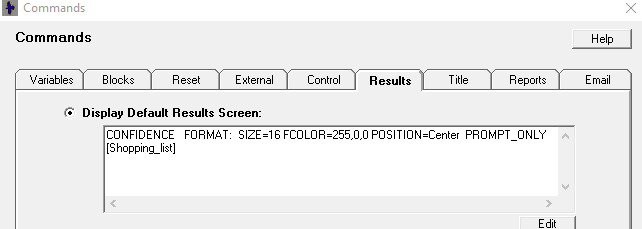
\includegraphics[width=0.9\linewidth]{bulb_11}
	\caption{Дополнительный вывод в результатах работы ЭС}
\end{figure}

\begin{figure}[H]
	\centering
	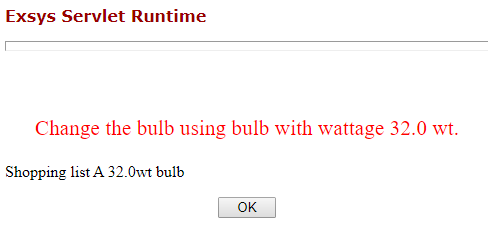
\includegraphics[width=0.7\linewidth]{bulb_12}
	\caption{Вывод ЭС с динамически формируемым списком покупок}
\end{figure}


Таким образом, было рассмотрено добавление в систему переменной типа \code{Collection} и ее вывод в качестве результата работы.

\newpage

\section{Разработка статической ЭС}

Разработаем статическую ЭС для прибора Диск-250 ДД.

\subsection{Переменные}

Разработанная система включает в себя переменные типа \code{Static list}, отражающие варианты сломанных частей прибора, и типа \code{Confidence}, использующиеся для рекомендации по починке прибора.

\begin{table}[H]
	\centering
	\caption{Список переменных}
	\begin{tabular}{|c|l|c|}
		\hline
		Тип                          & \multicolumn{1}{c|}{Название}   & Комментарий       \\ \hline
		\multirow{9}{*}{Static list}
		& \scode{Q_Problem}                                            & Disk problem is   \\ \cline{2-3} 
		& \scode{Q_Doesnt_work_when_turned_on}                         & Possible cause is \\ \cline{2-3} 
		& \scode{ Q_Fuse_box_burns_when_turned_on}                     & Possible cause is \\ \cline{2-3} 
		& \scode{Q_Pointer_goes_to_the_end_of_the_scale}               & Possible cause is \\ \cline{2-3} 
		& \scode{Q_The_motor_does_not_rotate}                          & Possible cause is \\ \cline{2-3} 
		& \scode{Q_Reversed_in_the_end_positions}                      & Possible cause is \\ \cline{2-3} 
		& \scode{Q_The_instrument_pointer_moves_slowly}                & Possible cause is \\ \cline{2-3} 
		& \scode{Q_Chart_disk_does_not_rotate}                         & Possible cause is \\ \cline{2-3} 
		& \scode{Q_The_readings_do_not_correspond_the_true_value}s     & Possible cause is \\ \hline
		\multirow{13}{*}{Confidence}
		& \scode{A_No_voltage_in_the_network}                          & 10                \\ \cline{2-3} 
		& \scode{A_Burned_insert_fusible}                              & 10                \\ \cline{2-3} 
		& \scode{A_Faulty_switch}                                      & 10                \\ \cline{2-3} 
		& \scode{A_Short_circuit}                                      & 10                \\ \cline{2-3} 
		& \scode{A_Rheochord_terminals_are_not_connected_correctly}    & 10                \\ \cline{2-3} 
		& \scode{A_Faulty_kinematic_system}                            & 10                \\ \cline{2-3} 
		& \scode{A_An_open_in_the_windings}                            & 10                \\ \cline{2-3} 
		& \scode{A_The_capacitor_shunting_the_motor_winding_is_faulty} & 10                \\ \cline{2-3} 
		& \scode{A_No_voltage_on_the_control_winding}                  & 10                \\ \cline{2-3} 
		& \scode{A_Polluted_rheohord}                                  & 10                \\ \cline{2-3} 
		& \scode{A_Mashing_in_the_kinematic_chain}                     & 10                \\ \cline{2-3} 
		& \scode{A_Motor_defective}                                    & 10                \\ \cline{2-3} 
		& \scode{A_Faulty_sensor_or_connecting_wires}                  & 10                \\ \hline
	\end{tabular}
\end{table}

\subsection{Дерево решений ЭС}

Приведем дерево решений разработанной ЭС.

\begin{figure}[H]
	\centering
	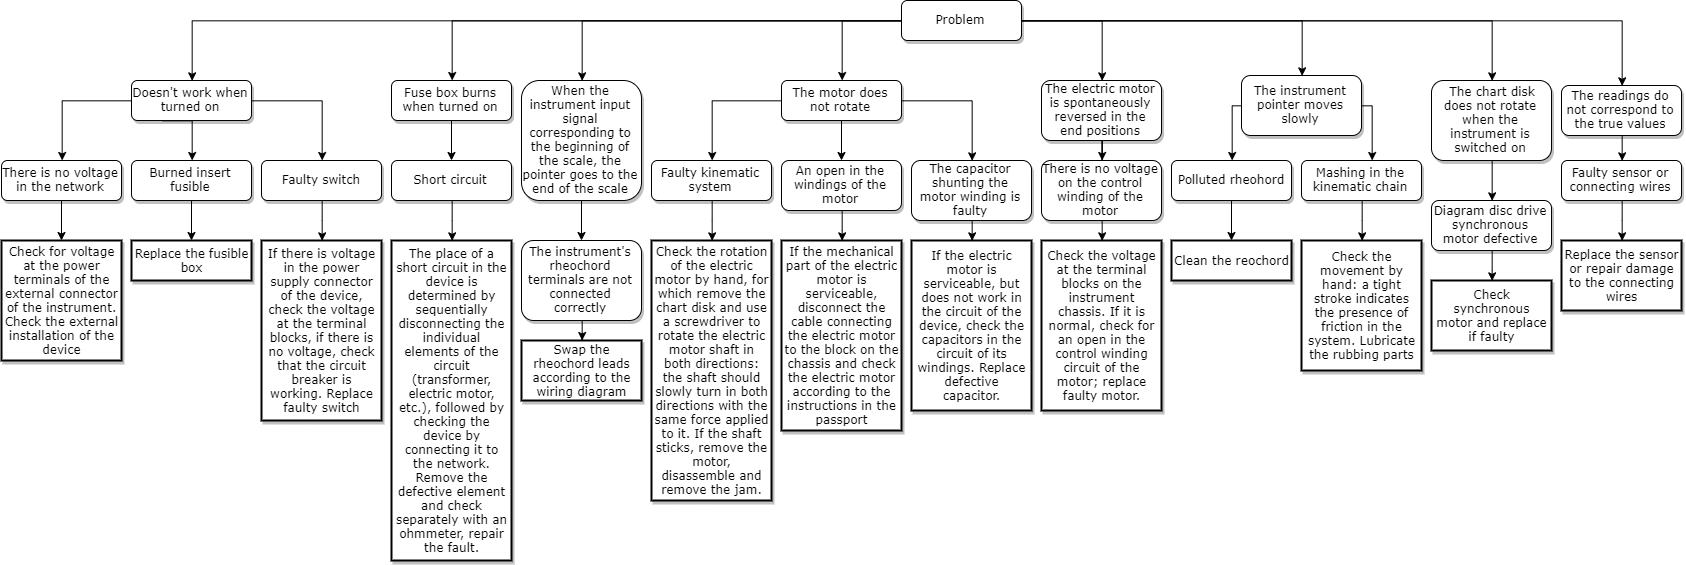
\includegraphics[height=0.45\linewidth,angle=-90]{tree}
	\caption{Дерево решений ЭС}
\end{figure}

\subsection{База знаний ЭС}

Приведем описание логического блока ЭС.

\begin{lstlisting}[caption={Алгоритм работы ЭС}]
IF:
	Disk's problem is Doesnt work when turned on
AND:
	Possible cause is There is no voltage in the network
THEN:
	Check for voltage at the power terminals of the external connector of the instrument. Check the external installation of the device: Confidence = 10

IF:
	Disk's problem is Doesnt work when turned on
AND:
	Possible cause is Burned insert fusible
THEN:
	Replace the fusible box: Confidence = 10

IF:
	Disk's problem is Doesnt work when turned on
AND:
	Possible cause is Faulty switch
THEN:
	If there is voltage in the power supply connector of the device, check the voltage at the terminal blocks, if there is no voltage, check that the circuit breaker is working. Replace faulty switch: Confidence = 10

IF:
	Disk's problem is Fuse box burns when turned on
AND:
	Possible cause is Short circuit
THEN:
	The place of a short circuit in the device is determined by sequentially disconnecting the individual elements of the circuit (transformer, electric motor, etc.), followed by checking the device by connecting it to the network. Remove the defective element and check separately with an ohmmeter, repair the fault.: Confidence = 10

IF:
	Disk's problem is When the instrument input signal corresponding to the beginning of the scale, the pointer goes to the end of the scale
AND:
	Possible cause is The instrument's rheochord terminals are not connected correctly
THEN:
	Swap the rheochord leads according to the wiring diagram: Confidence = 10

IF:
	Disk's problem is The motor does not rotate
AND:
	Possible cause is Faulty kinematic system
THEN:
	Check the rotation of the electric motor by hand, for which remove the chart disk and use a screwdriver to rotate the electric motor shaft in both directions: the shaft should slowly turn in both directions with the same force applied to it. If the shaft sticks, remove the motor, disassemble and remove the jam.: Confidence = 10

IF:
	Disk's problem is The motor does not rotate
AND:
	Possible cause is An open in the windings of the motor
THEN:
	If the mechanical part of the electric motor is serviceable, disconnect the cable connecting the electric motor to the block on the chassis and check the electric motor according to the instructions in the passport: Confidence = 10

IF:
	Disk's problem is The motor does not rotate
AND:
	Possible cause is The capacitor shunting the motor winding is faulty
THEN:
	If the electric motor is serviceable, but does not work in the circuit of the device, check the capacitors in the circuit of its windings. Replace defective capacitor.: Confidence = 10

IF:
	Disk's problem is The electric motor is spontaneously reversed in the end positions
AND:
	Possible cause is There is no voltage on the control winding of the motor
THEN:
	Check the voltage at the terminal blocks on the instrument chassis. If it is normal, check for an open in the control winding circuit of the motor; replace faulty motor.: Confidence = 10

IF:
	Disk's problem is The instrument pointer moves slowly
AND:
	Possible cause is Polluted rheohord
THEN:
	Clean the reochord: Confidence = 10

IF:
	Disk's problem is The instrument pointer moves slowly
AND:
	Possible cause is Mashing in the kinematic chain
THEN:
	Check the movement by hand: a tight stroke indicates the presence of friction in the system. Lubricate the rubbing parts.: Confidence = 10

IF:
	Disk's problem is The chart disk does not rotate when the instrument is switched on
AND:
	Possible cause is Diagram disc drive synchronous motor defective
THEN:
	Check synchronous motor and replace if faulty: Confidence = 10

IF:
	Disk's problem is The readings do not correspond to the true values
AND:
	Possible cause is Faulty sensor or connecting wires
THEN:
	Replace the sensor or repair damage to the connecting wires.: Confidence = 10
\end{lstlisting}

\newpage

\subsection{Пользовательский интерфейс}

Для ЭС был разработан интерфейс, схожий с примерами из лабораторных работ.

\begin{figure}[H]
	\centering
	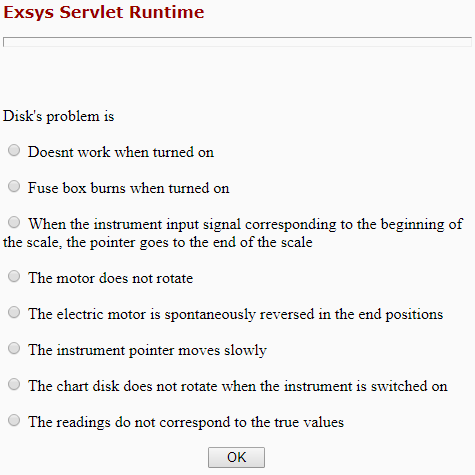
\includegraphics[width=0.7\linewidth]{disk_1}
	\caption{Пример задаваемого пользователю вопроса}
\end{figure}

\begin{figure}[H]
	\centering
	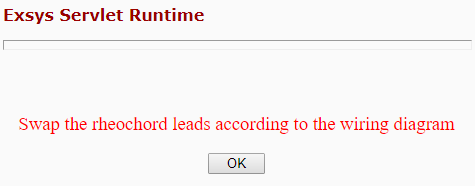
\includegraphics[width=0.7\linewidth]{disk_2}
	\caption{Пример результата работы ЭС}
\end{figure}

\newpage

\section{Выводы}

В рамках лабораторной работе была использована оболочка ExSys Corvid. Экспертные системы на базе этой оболочки используют правила \code{if}-\code{then}. В работе спроектирована простейшая экспертная система для замены лампочки в комнате и система поиска метода решения неисправностей прибора Диск-250 ДД.

Оболочка Corvid позволяет создавать переменные разных типов с указанием их значений; логические блоки, представляющие собой базу знаний; а также блок команд для запуска системы и представления результатов работы. Для созданной экспертной системы формируется пользовательский интерфейс, отображаемый в окне браузера.

\bibliographystyle{plain}
\addcontentsline{toc}{section}{Список литературы}
\bibliography{refs}

\end{document}
